
%%%%%%%%%%%%%%%%%%%%%%% file typeinst.tex %%%%%%%%%%%%%%%%%%%%%%%%%
%
% This is the LaTeX source for the instructions to authors using
% the LaTeX document class 'llncs.cls' for contributions to
% the Lecture Notes in Computer Sciences series.
% http://www.springer.com/lncs       Springer Heidelberg 2006/05/04
%
% It may be used as a template for your own input - copy it
% to a new file with a new name and use it as the basis
% for your article.
%
% NB: the document class 'llncs' has its own and detailed documentation, see
% ftp://ftp.springer.de/data/pubftp/pub/tex/latex/llncs/latex2e/llncsdoc.pdf
%
%%%%%%%%%%%%%%%%%%%%%%%%%%%%%%%%%%%%%%%%%%%%%%%%%%%%%%%%%%%%%%%%%%%


\documentclass[runningheads,a4paper]{llncs}

\usepackage{amssymb}
\setcounter{tocdepth}{3}
\usepackage{graphicx}
\usepackage{float}
\usepackage[full]{complexity}
\usepackage{amsmath}
%\usepackage{amsfonts}
%\usepackage{amsthm}
\usepackage{subfigure}
%\usepackage{caption}
%\usepackage{subcaption}
%\usepackage{cite}
\usepackage{hyperref}
\usepackage{url}
%\usepackage{clrscode4e}
\usepackage{verbatim}
\urlstyle{same}
\newcommand{\keywords}[1]{\par\addvspace\baselineskip
\noindent\keywordname\enspace\ignorespaces#1}

% Uniform numbering for previously defined theorem environments (e.g., LNCS).
\makeatletter
\let\c@lemma=\c@theorem
\let\c@corollary=\c@theorem
\let\c@fact=\c@theorem
\makeatother

% Redefinition of LNCS or SODA or Springer proof environment to put a \Box at
% the end of every proof.
\let\realendproof=\endproof
\def\endproof{\hspace*{\fill}$\Box$\realendproof}

\begin{document}

\mainmatter  % start of an individual contribution

% first the title is needed
\title{The Fewest Clues Problem}

% a short form should be given in case it is too long for the running head
\titlerunning{The Fewest Clues Problem}

% the name(s) of the author(s) follow(s) next
%
% NB: Chinese authors should write their first names(s) in front of
% their surnames. This ensures that the names appear correctly in
% the running heads and the author index.
%
\author{Erik D. Demaine \and Fermi Ma \and Ariel Schvartzman \and Erik Waingarten}
%
\authorrunning{Fermi Ma \and Ariel Schvartzman \and Erik Waingarten}
% (feature abused for this document to repeat the title also on left hand pages)

% the affiliations are given next; don't give your e-mail address
% unless you accept that it will be published
\institute{MIT,\\
77 Mass Ave., Cambridge, MA 02139, USA, \\
\protect\url{{edemaine,fermima,arielsc,eaw}@mit.edu}}

%
% NB: a more complex sample for affiliations and the mapping to the
% corresponding authors can be found in the file "llncs.dem"
% (search for the string "\mainmatter" where a contribution starts).
% "llncs.dem" accompanies the document class "llncs.cls".
%

\maketitle

\begin{abstract}
We study the problem of finding the fewest number of clues needed for a particular puzzle to be unique. We define a general transformation from search problems to fewest clues problems. We explore how the computational complexity of the problems change when we apply the transformation. We define two types of reductions relating fewest clues problems, and we show various \NP-complete problems have fewest clues versions which are $\Sigma_2$-complete. This line of research is similar to exploring the power of counting, as in \#P and ASP (another solution problem).
\end{abstract}

\section{Introduction}
\label{sec:introduction}

In 2012, McGuire, Tugermann, and Civario confirmed the conjecture that there are no uniquely solvable 16-clue Sudoku puzzles \cite{mcguire2012there}. It had long been known that 17 clues were sufficient. There exists an online database containing over 50,000 such puzzles. Thus, the result by McGuire et al. completely solves the problem of determining the minimum number of Sudoku clues needed. They arrived at this answer following a year-long computation. Is there any notion of computatational hardness to these sorts of problems?

We consider a following generalization of the above Sudoku question: 
\begin{quote}
For any given problem, what is the fewest number of clues necessary to make it uniquely solvable?
\end{quote}

For example, if the problem is to find a Hamiltonian cycle in a given graph $G = (V,E)$, our question would be to determine the minimum number of edges you must specify before only one Hamiltonian cycle contains all of these edges. This general problem is motivated by possible applications to puzzle-making. 

A puzzle-maker for a newspaper might want to make a puzzle that contains as few clues as possible, but is still uniquely solvable (as the puzzle-maker might want to publish the answer in the next day's paper). The input to the problem is an idea of a partially filled puzzle, and the output is the least number of additional clues needed for the puzzle to be uniquely solvable.

We formalize this problem by defining the ``Fewest Clues Problem" ($\mathsf{FCP}$). We treat $\mathsf{FCP}$ as a transformation of problems. We use this framework to analyze the $\mathsf{FCP}$ versions of classic $\NP$-hard problems such as SAT and 3SAT, as well as $\NP$-hard puzzle problems such as Latin square completion and Sudoku completion. We show that for many $\NP$-hard problems, their $\mathsf{FCP}$ versions are $\Sigma_2$-complete, and give examples problems with polynomial time algorithms whose $\mathsf{FCP}$ versions are $\Sigma_2$-complete.

The paper is organized as follows. In Section~\ref{sec:relatedwork}, we discuss previous research done on this problem for the specific cases of Sudoku, Latin Squares, and graph coloring. We note that while fewest clues problems has been studied extensively, it is almost always done so with respect to a certain problem. In Section~\ref{sec:prelim}, we motivate and formally define the transformation $\mathsf{FCP}$. We state what it means for a problem to be a fewest clues problem, and provide a framework for reducing between these problems. In Section~\ref{sec:The Problems}, we consider $\mathsf{FCP}$ versions of the SAT, 3SAT, Triangle Partition, Latin Squares and Sudoku completion problems, and show why these problems are $\Sigma_2$-complete. Then in Section~\ref{sec:easyproblems} we discuss how the $\mathsf{FCP}$ transformation affects problems with polynomial time algorithms. Finally, in Section~\ref{sec:conclusion} we give concluding remarks and ideas for further research.

\section{Related Work}
\label{sec:relatedwork}

Our work touches upon three major areas: Another Problem Solution, boolean formula minimization, and critical sets. 

\subsection{The Another Solution Problem ($\mathsf{ASP}$)}

Our approach the $\mathsf{FCP}$ transformation is related to the \emph{Another Solution Problem} ($\mathsf{ASP}$) \cite{Seta01}. For a given problem, the $\mathsf{ASP}$ version asks: given an instance and a solution for that instance, find another solution for that instance. There is a notion of an $\mathsf{ASP}$-reduction, defined in \cite{Seta01}. If $\mathsf{ASP} A$ can be $\mathsf{ASP}$-reduced to $\mathsf{ASP} B$, then $\mathsf{NP}$-hardness of $\mathsf{ASP} A$ implies $\mathsf{NP}$-hardness of $\mathsf{ASP} B$. In a follow-up paper, \cite{takayuki2003complexity} shows $\mathsf{ASP}$-completeness of Slither Link, Sudoku (or Number Place), and Fillomino. We use a similar approach to analyzing hardness of $\mathsf{FCP}$-hard problems. 

We consider the $\mathsf{FCP}$ version of the boolean satisfiability problem ($SAT$), and show that it is $\Sigma_2$-complete. We then define an $\mathsf{FCP}$-reduction similar in flavor to an $\mathsf{ASP}$-reduction, and show $\Sigma_2$-completenss of various $\mathsf{FCP}$ problems with these reductions.

\subsection{Boolean Formula Minimization}

Our approach to showing $\Sigma_2$-hardness of boolean formula minimization has many connections to boolean formula minimization. \cite{umans}\cite{umans2001minimum} explores the problem of Minimum Equivalent Expression and Shortest Implicant. The problem is very similar to the problem we consider when applied to SAT. In the shortest implicant problem, they ask for the minimum number of variables needed so that the formula is always satisfiable, no matter what assignment the other variables receive. They show this problem is $\Sigma_2$-complete.  

\subsection{Critical Sets}

Another line of research which is also very similar has been that of determining the size of critical sets. \cite{Cooper:2014:CSS:2612293.2612628} defines critical sets in much the same way we do; determining the fewest number of clues needed to obtain a unique solution. They focus on colorings on graphs. They can think of the Sudoku graph. This is a graph with $n^2$ vertices (one for each square), which has edges between vertices whose corresponding squares cannot be the same values. They ask for the smallest number of vertices needed to color in order for the remaining graph to have a unique $n$ color coloring. This is phrasing the problem of \cite{mcguire2012there} in graph and coloring notation. 

They prove some results regarding the sizes of critical sets for graph colorings and show that the problem is $\NP$-hard. Our results improve on these results by showing that these graph colorings are in fact $\Sigma_2$-complete, which fully characterizes their complexity.

\cite{Ghandehari2005121} did a similar type of analysis, where they bound the size of the smallest critical set for Latin Squares. \cite{colbourn1984computational} also analyzes the complexity of recognizing critical sets. They ask exactly the ASP question for Latin Squares, and show it is $\NP$-complete.



\section{The $\mathsf{FCP}$ Transformation}
\label{sec:prelim}

\subsection{Definitions}

For a given instance of $x$ of a \emph{search} problem A, we can think of the set of solutions to $x$ as a set of polynomial-size strings. For example, for the case of $SAT$, an instance consists of a specific $SAT$ formula on variables $x_1,x_2,\dots,x_n$. Solutions can be written as indexed length-$n$ strings of boolean values, where the value at index $i$ is the assignment to variable $x_i$. In this case, a $\emph{clue}$ for the problem would be an assignment of a specific index to some boolean value. For general problems, the precise definition of a clue depends on how solutions are encoded as strings.

We say that a solution to $x$ \emph{satisfies} a set of clues if each clue matches the solution at that clue's index. For example, in the case of SAT on variables $x_1,x_2,\dots,x_5$, then the solution $``01011"$ would match the clue set $\{x_1 = 0,x_3 = 0,x_4 = 1\}$.

Given these definitions, we define $\mathsf{FCP} A$ to be the following decision problem:
\begin{quote}
Given $A$ and a valid encoding of solutions of $A$, is there a set of clues of size at most $k$ such that exactly one solution satisfies these clues?
\end{quote}
%
%In particular, we will have an $\NP$ search problem be comprised of a set of \emph{instances}, which will be strings over some finite alphabet. For a particular instance $x$, there is set of possible \emph{solutions}, which are strings of polynomial size with respect to $|x|$ over some finite alphabet. Each problem also comes with an algorithm $A$ that checks whether a string $s$ is in fact a solution for an instance $x$, which runs in polynomial time. This is the verifier. For a given language $L \in \NP$, $x \in L$ if and only if $S(x)$ is non-empty.
%
%A \emph{clue} will be an indexed character of a solution. So a clue indicates what character lies at some position of the solution.
%
%\begin{definition}
%Given some $\NP$ search problem $A$, the ``fewest clues" version of $A$, $(\mathsf{FCP} A)$ asks for an instance of $A$, the minimum number of clues corresponding to a unique solution for any given instance?
%\end{definition}

This set-up allows us to ask $\mathsf{FCP}$ variations to the common puzzles like Sudoku quite easily. For the classical $9 \times 9$ Sudoku, we let the alphabet be $\Sigma = \{ 1, ..., 9 \} \cup \{ \Box \}$, and we let an instance be a string of length 81 with elements from $\Sigma$, where each position in the string corresponds to a position on the $9 \times 9$ Sudoku board. The presence of $\Box$ indicates that position is unknown. A solution will be a string of length $81$ with no $\Box$ characters. 

The algorithm $A$ checks whether a solution to some instance is correct. It does so by checking all three Sudoku rules: every row, column, and $3 \times 3$ inner-square contains all the numbers from $\{1 , ..., 9\}$. In addition, we check the solution contains the same numbers as the instance at the specified positions.

\begin{figure}
\centering
\label{fig:seventeencluesudoku}
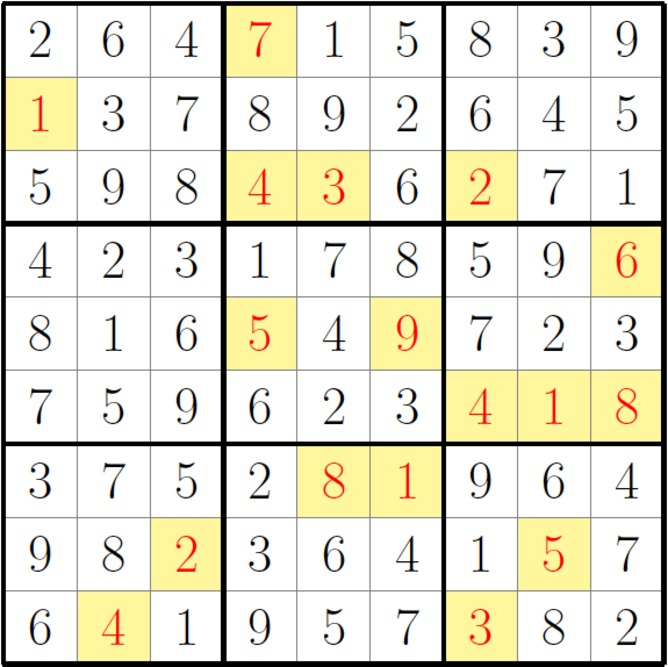
\includegraphics[width=0.5\linewidth]{seventeencluesudoku.jpg}
\caption{17-Clue $9 \times 9$ Sudoku, taken from \cite{smallsudoku}}
\end{figure}

$\mathsf{FCP}$ Sudoku asks for a given starting point $x$ which is the fewest number of additional squares we must fill in order for the Sudoku to be uniquely solvable. A solution for the $9 \times 9$ case where the instance is initially empty is given in Figure~\ref{fig:seventeencluesudoku}. The fewest clues are given by the yellow squares.

\subsection{Upper Bounds}

Usually, we will talk about $\NP$ search problems which we transform to $\mathsf{FCP}$ versions. We can obtain an immediate upper bound.

\begin{theorem}
\label{thm:satinsig2}
If some language $L \in \NP$, then $\mathsf{FCP} L \in \Sigma_2$. 
\end{theorem}

\begin{proof}
We can write the $\mathsf{FCP}$ question in terms of a $\Sigma_2$ question. The original $\NP$ question for $L$ is
\[ x \in L \leftrightarrow \exists y, A(x, y) = 1 \]
For some polynomial time algorithm $A$. The corresponding $\mathsf{FCP} L$ question is
\[ (x, k) \in \mathsf{FCP} L \leftrightarrow \exists c_y, y \forall y' A'(x, c_y, y, y') = 1 \]
Where $A'$ checks that $c_y \subset y$, that $c_y \subset y' \neq y$, and that $A(x,y) = 1$, $A(x, y') = 0$ and that $|c_y| \leq k$. In other words, $c_y$ is a clue of $y$, and $y'$ is another solution. $A'$ checks that $c_y$ has at most $k$ elements, and that it is a clue of the solution $y$, and that there are no other solutions. 
\end{proof}

We could generlize our statement a bit. The above proof says that if $L \in NTIME[f(n)]$, then $\mathsf{FCP} L \in \Sigma_2 NTIME[f(n)]$, when $f(n) > n$. 

\subsection{$\mathsf{FCP}$ SAT}

The $\mathsf{FCP}$ SAT problem is the following:
\begin{quote}
\textbf{Instance}: A Boolean formula $\phi$, and a number $k$.\\
\textbf{Question}: Does there exists a partial assignment of at most $k$ variables such that the remaining formula $\phi'$ has only one satisfying assignment?
\end{quote}

From Theorem~\ref{thm:satinsig2}, we know that $\mathsf{FCP}$ SAT $\in \Sigma_2$. We now wish to show that $\mathsf{FCP}$ SAT is $\Sigma_2$-complete. We take the following $\Sigma_2$ complete problem: QSAT 
\begin{quote}
\textbf{Instance}: $\phi$ a Boolean function on $x$ and $y$ sets of variables. \\ 
\textbf{Question}: Does there exists a setting of the $x$ variables, such that for all the setting of the $y$ variables, $\phi(x,y) = 0$? Equivalently,$\exists x \forall y \phi(x,y) = 0$?
\end{quote}
We will write this problem as an equivalent $\mathsf{FCP}$ SAT question.

First, we take add a unique solution. We look at the modified question, $UQSAT$:
\begin{quote} 
\textbf{Instance}: A Boolean formula $\phi$ on $x$ and $y$ sets of variables. \\
\textbf{Question}: Does there exists a setting of the variables in $x$ such that $phi(x)$ has a unique solution on the $y$'s?
\end{quote}

\begin{lemma}
$UQSAT$ is $\Sigma_2$-hard.
\end{lemma}

\begin{proof}
We will want to reduce from $QSAT$. We do this by starting with the expression $\phi(x,y)$ and transform it into an expression $\phi'(x, y, z)$, where $z$ is an additional variable. We show
\[ \exists x \forall y \phi(x,y) = 0 \leftrightarrow \exists x \forall y\cup \{z\} \left(\phi'(x, 0, 0) = 1 \right) \wedge \left((y \neq 0 \vee z \neq 0 ) \rightarrow \phi'(x, y, z) = 0 \right). \]
The expression $\phi'(x, 0, 0)$ corresponds to setting all variables in $y$ to $0$ as well as $z$ to 0. The expression $y \neq 0$ is short-hand for $\bigvee_{y_i \in y} y_i \neq 0$. 

The left-hand side is $QSAT$. The right-hand side says that once we set $x$, $\phi'$ has only one solution at $y=0$ and $z = 0$. Running $UQSAT$ on $\phi'$ with variables $x$ and $y \cup \{z\}$ will be true if and only if $QSAT$ on $\phi$, $x$ and $y$ is true. Therefore, showing the above expression is true proves the lemma.

We let 
\begin{align}
\phi'(x, y, z) &= C_1 \vee C_2 \\
		    C_1 &=\left(\phi(x, y) \wedge (z = 1)\right) \\
		   C_2 &=  \left( y = 0 \wedge z = 0 \right) 
\end{align}
Note that $\phi'(x, 0, 0) = 1$. If $\exists x \forall y \phi(x, y)= 0$, then there is a setting of $x$ such that the $C_1 = 0$. The only way to satisfy $\phi'$ is through setting $y = 0$ and $z = 0$. If for any setting of $x$, there exists a setting of $y$ such that $\phi(x, y) = 1$, then we have some setting of $\phi'(x, y, 1) = 1$. So $UQSAT$ would also be false since that assignment as well as $x, 0, 0$ evaluate to true.
\end{proof}

\begin{proposition}
\label{prop:fcpsatsigmacomp}
$\mathsf{FCP} $SAT is $\Sigma_2$-hard.
\end{proposition}

\begin{proof}
We will reduce from $UQSAT$. For a given $\phi(x, y)$ with $|x| = k$, we ask, does there exists a setting of $2k$ variables such that $\phi'(x, x', y) = \phi(x, y) \vee \bigvee_i (x_i = x_i')$ has a unique solution?

First we prove one direction: $\exists x$ such that $\phi(x,y)$ has a unique satisfying assignment on $y$'s implies that $\exists x, x'$ such that $\phi'(x,x',y)$ has a unique satisfying assignment on $y$'s.
Suppose $\exists x$ such that $\phi(x,y)$ has a unique satisfying assignment on $y$'s. Let $\hat{x}$ be the one such assignment on $x$. Let $x = \hat{x}$, and for all $i$, we let $x_i' \neq x_i$. The remaining formula $\phi'(x, x', y)$ on $y$s has a unique solution. This is because once we set $x$ and $x'$, 
\[ \phi(x, y) \leftrightarrow \phi'(x,x',y) \]

Now we prove the other direction: If for every $x$, $\phi(x,y)$ does not have a unique solution on the $y$'s, then for any assignment of $2k$ variables, $\phi'(x,x',y)$ does not have a unique solution on the remaining variables. 
Suppose for any setting of $x$, there is more than one setting of $y$s with a satisfying assignment. In other words, $\phi(x, y) \notin UQSAT$. Let $C$ be a set of variable assignments, where $|C| \leq 2k$. If $x, x' \subset C$, then we know that for all $i$, $x_i \neq x_i'$. If they were for one such $i$, then any other assignment on the remaining variables will satisfy $\phi'(x,x',y)$. Furthermore, there will be more than one setting of $y$'s to satisfy $\phi'(x,x',y)$ since multiple $y$'s can satisfy $\phi(x,y)$. However, if some $y_i \in y$ is set, so $y \cap C \neq \emptyset$, there will be some $x_i$ or $x_i'$ not in $C$. Setting $x_i = x_i'$ will allow an arbitrary setting of the remaining variables. $\phi'$ therefore does not have a unique satisfying assignment. If $\phi(x,y)$ has no satisfying assignment, then $\phi'(x,x',y)$ has either 0 or many satisfying assignments. This finishes the reduction.
\end{proof}

Having shown that $\mathsf{FCP}$ SAT is $\Sigma_2$-complete, we will be able to reduce $\mathsf{FCP}$ problems to $\mathsf{FCP}$ SAT.

\section{Complete Problems}
\label{sec:The Problems}

\subsection{Reductions}

We define a special type of reductions that will allow us to reduce between $\mathsf{FCP}$ problems. This will make it easy to show that certain $\mathsf{FCP}$ versions of $\NP$-complete problems are $\Sigma_2$-complete by using their Karp style reductions and showing that they satisfy additional properties. We formalize this notion with the General Clue Reduction.

\subsubsection{General Clue Reduction}

\begin{definition}
Suppose $A$ and $B$ are problems with instance sets $I_A$ and $I_B$ and clue sets $C_A$ and $C_B$. We say $A$ reduces to $B$ via a general clue reduction if
\begin{enumerate}
\item We have $f: I_A \rightarrow I_B$ where $x \in A \iff f(x) \in B$.
\item We have $g: C_B \rightarrow C_A$ such that:
\begin{itemize}
\item $g$ is surjective. 
\item $g$ is a bijection on solutions.
\item $c \subset c' \Rightarrow g(c) \subset g(c')$. In addition, if $g(c) \subset S$ is a solution of $x \in A$, then $c \subset g^{-1}(S')$.
\item $|c| \geq |g(c)|$, with equality for minimal clues. 
\end{itemize}
\end{enumerate}
\end{definition}
Note that $f$ is the usual notion of reduction. We add $g$ so that we can map minimal clues to minimal clues. Once we have a general clue reduction from $A$ to $B$, then we solve $\mathsf{FCP} A$ using $\mathsf{FCP} B$. On input $x \in I_A$:
\begin{enumerate}
\item Let $f(x)$ be the instance of $B$ mapped by the reduction.
\item Find a minimal clue for $f(x)$, $c_{f(x)}$. 
\item Use $g: C_B \rightarrow C_A$ to get the clue $g(c_{f(x)})$ of $x$.
\end{enumerate}

\begin{lemma}
Let $x \in I_A$ and $f$, $g$ and $c_{f(x)}$ be as defined above. Then $g(c_{f(x)})$ is a minimal clue set for instance $x$.
\end{lemma}

\begin{proof}
We want to show that if $c_{f(x)}$ is a minimum clue set, then $g(c_{f(x)})$ is a minimum clue set as well. We need to fullfill three conditions:
\begin{enumerate}
\item $g(c_{f(x)})$ is a clue of $x$. 
\item $g(c_{f(x)})$ has a unique superset solution.
\item $g(c_{f(x)})$ is minimal.
\end{enumerate}

1. $c_{f(x)}$ is a clue for $f(x)$, so $c_{f(x)} \subset S_{f(x)}$ for some solution $S_{f(x)}$. 
\begin{align} c_{f(x)} \subset S_{f(x)} \Rightarrow g(c_{f(x)}) \subset g(S_{f(x)}) \end{align}
Since $g$ preserves subsets.

2. If $g(c_{f(x)})$ had two different solutions, $S_x^{(1)}, S_x^{(2)}$, 
\begin{align}
g(c_{f(x)}) \subset S_x^{(1)}&& g(c_{f(x)}) \subset S_x^{(2)} \\
c_{f(x)} \subset g^{-1}(S_x^{(1)}) && c_{f(x)} \subset g^{-1}(S_x^{(2)})
\end{align}
Since $g^{-1}$ preserves subsets on solutions. So $c_{f(x)}$ would have two different solutions.

3. Suppose $|g(c_{f(x)})|$ is not minimal. Let $c_x$ be the minimal clue for $x$. So $|c_x| < |g(c_{f(x)})|$. $g$ is surjective, so let $c' \in C_B$ with $g(c') = c_x$. So $|c'| < |c_{f(x)}|$. $c_{f(x)}$ is a minimal clue for $f(x)$ by assumption. Therefore, either $c'$ has no solution, or more than one solution. We know that $c'$ has at least one solution since $c_x$ has a solution, and $g^{-1}$ is a bijection and maintains subsets. If $c'$ had two solutions, then $c_x$ would have two solutions. Therefore, $|g(c_{f(x)})|$ is minimal.
\end{proof}

\begin{corollary}
\label{thm:reduction}
Suppose $A$ reduces to $B$ with a general clue reduction and $\mathsf{FCP} A$ is $\Sigma_2$-hard, then $\mathsf{FCP} B$ is $\Sigma_2$-hard. 
\end{corollary}

One downside to the General Clue Reduction is that it requires the solutions to the problems to be in bijection. In general, this constraint is too strong, so we define a different kind of reduction which will have more requirements, but which will apply to a greater variety of cases.

\subsubsection{Special Subset Clue Reduction} This will be similar to the General Clue reduction, except we only look at a particular subset of clues.

We will first need a function $f: I_A \rightarrow I_B$ such that $x \in I_A$ has a solution if and only if $f(x) \in I_B$ has a solution. We additionally specify $C_B' \subset C_B$ and an algorithm $M$ that maps any minimal clue set in $C_B$ into a minimal clue set in $C_B'$ of the same size which runs in polynomial time. We will now let $g: C_B' \rightarrow C_A$ which satisfies the following properties:
\begin{enumerate}
\item $g$ is surjective.
\item $g$ is a bijection on solutions, and $S_x$ is a solution for $x$, if and only if $g^{-1}(S_x)$ is a solution to $f(x)$. 
\item $c \subset c' \Rightarrow g(c) \subset g(c')$ and if $g(c) \subset S$, then $c \subset g^{-1}(S)$.
\item $|c| \geq |g(c)|$, with equality for minimal clues.   
\end{enumerate} 
This type of reduction generalizes the General Clue Reduction, since we can specify a special subset of clues. Given a reduction, we can solve an instance $x$ of $A$ in the following manner:
\begin{enumerate}
\item Let $f(x)$ be the instance of $B$ mapped by the reduction.
\item Find a minimal clue for $f(x)$, $c_{f(x)}$. 
\item Apply $M$ to $c_{f(x)}$ to get $c_{f(x)}' \in C_B'$. 
\item Use $g: C_B' \rightarrow C_A$ to get the clue $g(c_{f(x)}')$ of $x$.
\end{enumerate}

A Special Subset Clue Reduction is like a General Clue Reduction. We restrict the problem to have a specific kind of clues, and we give a way to tranform the clues. 

\begin{corollary}
\label{thm:special_reduc}
Suppose $A$ reduces to $B$ with a special subset clue reduction and $\mathsf{FCP} A$ is $\Sigma_2$-hard, then $\mathsf{FCP} B$ is $\Sigma_2$-hard. 
\end{corollary}

\subsection{3SAT}

\begin{theorem}
$\mathsf{FCP}$ 3SAT is $\Sigma_2$-complete. 
\end{theorem} 

\begin{proof}
We reduce from $\mathsf{FCP}$ 3SAT via a general clue reduction. We will define a recursive mapping $f$ from instances of SAT to those of 3SAT. Suppose we are given a SAT formula $\phi$ with clauses $C_i$. If $|C_i| \leq 3$, then we preserve the clause. Otherwise, if $C_i$ has $k$ variables $x_1,...,x_k$ we replace the original clause with 
\[ 
(x_1 \vee x_2 \vee z_2) \wedge (\overline{z_2} \vee \overline{x_2}) \wedge (z_2 \vee x_2) \wedge f(\overline{z_2}, x_3, ..., x_k) 
\]

where the last term indicates we keep recursing until each clause has at most $3$ variables. Note that on each step we reduce the number of variables in the longest clause by at least $1$, so after $O(n)$ steps (per clause) we will have a valid 3SAT instance at the cost of adding variables and small clauses. It is not hard to see that the original clause and it's mapped version agree on solutions. Notice that by construction $x_i \leftrightarrow \overline{z_i}$. 

Now I will define $g$. $g$ will take a clue for 3SAT, or a partial assignment of the variables in $f(\phi)$ and give a partial assignment of the variables in $\phi$, it does this by mapping each variable individually. $g$ is the identity on the $x_i$ variables, and $g$ maps $z_i$ to $\overline{x_i}$. We check the properties of $g$:
\begin{enumerate}
\item $g$ is surjective. If there is any clue of $\phi$, it is also a clue of $f(\phi)$. 
\item $g$ is bijective on solutions. An assignment of $f(\phi)$ gives the assignment for $\phi$, and that same assignment uniquely describes the assignments for $z_i$, so $g$ bijectively maps them.
\item $g$ maps variables to variables, so $c \subset c' \Rightarrow g(c) \subset g(c')$. If $g(c) \subset S$, then $c \subset g^{-1}(S)$. 
\item $|c| \geq |g(c)|$ since for each variable in $c$, there is at most one variable in $g(c)$. The inequality becomes an equality for minimal clues since we will never have $x_i$ and $z_i$ in a minimal clue.
\end{enumerate}
\end{proof}

\begin{corollary}
Not-All-Equal 3SAT (NAE 3SAT) is $\Sigma_2$-complete.
\end{corollary}

\begin{proof}
The reduction for 3SAT above also works for NAE 3SAT. $x_i = \overline{z_i}$ which means that no satisfying assignment will have all three literals true in a clause. 
\end{proof}

\subsection{Triangle Partition}\label{S:TP}

The Triangle Partition problem is the following:
\begin{quote}
\textbf{Instance}: A undirected graph $G = (V, E)$.\\
\textbf{Question}: Can we partition $E$ into disjoint triangles?
\end{quote}

Holyer \cite{holyer1981np} showed this problem is $\NP$-complete. His main tool (shown in Figure~\ref{fig:holyergraph}) was the graph $H_{3, p}$, which has only two possible triangle partitions. Note this is a small section of the graph, and it continues with these type of tilings.
\begin{figure}
\label{fig:holyergraph}
\centering
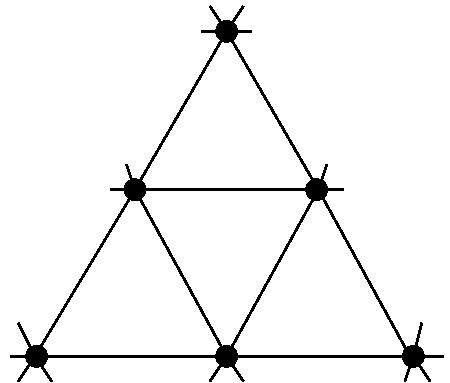
\includegraphics[width=0.4\linewidth]{Holyergraph.pdf}
\caption{Holyer's $H_{3,p}$ graph}
\end{figure}

The $\mathsf{FCP}$ version of the problem is to find the fewest number of triangles we must give in order for there to be a unique triangle partition. For example, in $H_{3,p}$ (Figure~\ref{fig:holyergraph}), once you specify one triangle in the partition, there is only one way to partition the graph in accordance with that triangle.

We claim $\mathsf{FCP}$ Triangle Partition is $\Sigma_2$-complete. We give a quick summary of Holyer's reduction which highlights the ideas we will use to show $\Sigma_2$ completeness. 

\subsubsection{Holyer's Reduction for Triangle Partition}
%
% Fermi, do you think we need both paragraph version of summary and important properties?
%
% 
Holyer uses the graph $H_{3,p}$ in Figure~\ref{fig:holyergraph} to represent variables and literals. Since each graph can only be partitioned in one of two ways, one way will correspond to a true setting, the other will correspond to a false setting. They call the two possible partitions the $T$-partition and the $F$-partition. 

\begin{figure}
\begin{minipage}{0.5\linewidth}
\centering
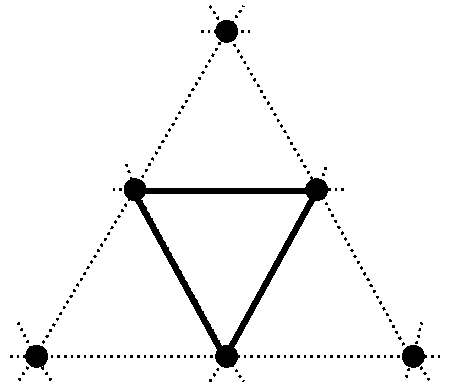
\includegraphics[scale=0.5]{Tpartition.pdf}
\label{fig:tpart}
\caption{$H_{3,p}$ partitioned like a $T$-partition. In a particular part of the graph, one triangle specified.}
\end{minipage}
\hfill
\begin{minipage}{0.5\linewidth}
\centering
\label{fig:fpart}
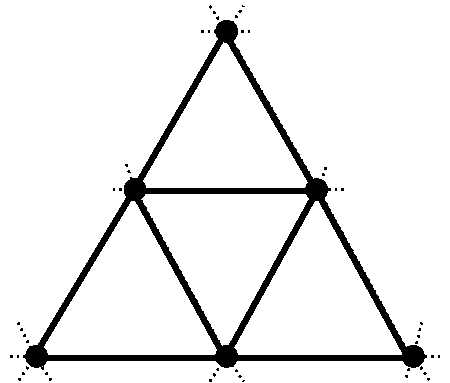
\includegraphics[scale=0.5]{Fpartition.pdf}
\caption{$H_{3,p}$ partitioned like an $F$-partition. In a particular part of the graph, three triangles specified.}
\end{minipage}
\end{figure}

The authors also use the graphs to make clauses. They show a way to join three $H_{3,p}$ graphs such that exactly one of them will be $F$-partitioned. The three graphs will correspond to literals in the clause. Then they give a way to combine the literals with the variables such that if a literal is set to an $F$-partition, then corresponding variable must be set to either a $T$-partition (in the case where the literal is positive), or an $F$-partition (if the literal is negative). However, if the literal is a $T$-partition, then it does not matter what the variable is set to. 

In particular, there are three important properties of Holyer's reduction which we utilize:
\begin{enumerate}
\item We have variable and literal gadgets which are a graph which can be partitioned in two possible ways, we call one $T$-partitioned (corresponding to setting the variable to true) and $F$-partitioned (corresponding to setting the variable to false).  
\item A clause gadget is a join between three literal gadgets. The clause gadget has a triangle partition if exactly one of the literals is $F$-partitioned.
\item A literal is joined with a variable. If the literal is $F$-partitioned, then there are two options:
\begin{itemize}
\item If the literal is the positive variable, then the variable must be $T$-partitioned.
\item If the literal is the negative variable, then the variable must be $F$-partitioned.
\end{itemize}
\end{enumerate}
So the argument is: if the graph can be triangle partitioned, then each clause is satisfied by at least one literal. That literal gadget will be $F$-partitioned and it will cause the variable to take a particular partition, giving it its assignment. 

\begin{theorem}
$\mathsf{FCP}$ Triangle Partition is $\Sigma_2$-complete.
\end{theorem}

\begin{proof}
We refer the reader to \cite{holyer1981np}, \cite{colbourn1984complexity} for questions about notation. We will show a special subset clue reduction from $\mathsf{FCP}$ 3SAT. 

We define $f$ to map instances of 3SAT to Triangle Partition as in \cite{holyer1981np}.

We let the special clue set $C_B'$ be the clues where if a triangle appears in a literal graph, then a triangle appears in a literal graph of the same clause which corresponds to an $F$-partition, and the $F$-partition corresponds to the first true literal.

The algorithm $M$: 
\begin{enumerate}
\item If we get a clue with a triangle in a literal corresponding to a $T$-partition, we exchange it with a triangle for a literal in the same clause corresponding to an $F$-partition. This does not change the solution since the $F$-partition triangle must appear and it implies the $T$-partition triangle. 
\item If the $F$-partition literal corresponds to the second or third true literal in the clause, then exchange it for the $F$-partition triangle corresponding to the first true literal in the clause. This changes the solution to the triangle partition, but doens't change the variable graphs, only that particular clause graph, and the solution is still unique.
\end{enumerate}

Now $g$ maps the triangles in variable graphs to the corresponding assignment and the $F$-partition literals to the correspoding variable assignments. We check the conditions for $g$.
\begin{itemize}
\item $g$ is surjective, since the variable assignments correspond to variable gadget partitions.
\item $g$ is a bijection on solutions, since once the variable graphs are partitioned, we force the first true literal to be $F$-partitioned. 
\item Since we are mapping individual triangles, subsets are preserved. $g(c) \subset S$, then $g^{-1}(S)$ presents a full triangle partition from $C_B'$, so $c \subset g^{-1}(S)$. 
\item We are projecting certain triangles to variables, so there is at most one variable per triangle. In minimal clue sets, we will need exactly one variable per triangle.
\end{itemize}
\end{proof}

\subsection{Latin Squares}

The Latin Squares problem is the following:
\begin{quote}
\textbf{Instance}: An $n \times n$ grid, with some entries filled in with the numbers $1$ to $n$.\\
\textbf{Question}: Can we fill in the remainder of the grid with numbers from $1$ to $n$ while enforcing that no row or column repeat a number?
\end{quote}
The problem was shown to be $\NP$-complete by Colbourn \cite{colbourn1984complexity}. Here, we study its  $\mathsf{FCP}$ version, which asks what is the fewest number of entries that must be filled in so the Latin Square becomes uniquely solvable. This problem is $\Sigma_2$-complete. 

\subsubsection{Colbourn's Reduction for Latin Squares:}
We give a quick summary of Colbourn's main ideas which will help the reader understand the $\Sigma_2$-completeness reduction. There are two main steps in his proof. In the first, Colbourn shows that completing partial Latin Squares is equivalent to partitioning tripartite graphs into triangles, a problem similar to the one in section \ref{S:TP} which they show is $\NP$-complete. In the second step, the authors use embedding techniques to reduce triangle partitions of tripartite graphs to Latin Square completion. 

Colbourn \cite{colbourn1984complexity} first argues that in order to decide whether or not a triangle partition exists on a tripartite graph it suffices to consider the cases where the graph is uniform. We say a tripartite graph $G = (V_1 \cup V_2 \cup V_3, E)$ is \emph{uniform} if any vertex $x \in V_1$ (symmetrically $V_2, V_3$) has the following property: it has the same number of neighbors on the other two parts of the partition. 

Throughout this section we refer to the entry on the $i$-th row and $j$-th column of a Latin Square as $L(i,j)$. The authors introduce the concept of a defect graph $G(P)$, a tripartite graph that has a triangle partition if and only if its originating Latin Square $P$ is completable. 

\begin{definition}
Suppose we are given a partial Latin Square $P$ of order $n$. The \textbf{defect graph $G(P) = (V,E)$} of $P$ is the graph whose vertex set is given by $$\{ r_i | \text{ row } i \text{ contains an empty square} \} \cup \{ c_j | \text{ column } j \text{ contains an empty square} \} $$
$$ \cup \{ e_k | \text{ element } k\text{ appears less than } n \text{ times } \} .$$ 

The edge set of $G(P)$ is defined as follows: 

\begin{itemize}
	\item If $L(i,j)$ is blank, then we add an edge between $r_i$ and $c_j$. 
	\item If row $i$ does not have item $k$ then we add an edge between $r_i$ and $e_k$. 
	\item If column $j$ does not have item $k$ then we add an edge between $c_j$ and $e_k$.
\end{itemize}
\end{definition}

Colbourn \cite{colbourn1984complexity} shows the following lemma: 
\begin{lemma}\label{TP:lemma}
A partially completed Latin Square $P$ has a valid solution if and only if its defect graph $G(P)$ has a triangle partition. 
 \end{lemma}
 
The authors show a modification of Holyer's proof that Triangle Parition is $\NP$-complete to show that finding a triangle partition of a tripartite graph is also $\NP$-complete. They make some minor modifications which force the graph to be tripartite. These modifications can be found in \cite{colbourn1984complexity} and do not affect the $\Sigma_2$-completeness proof above. 

Next, Colbourn shows the reduction between the problem of finding triangle partitions in tripartite graphs and Latin Squares completion by introducing the concept of a Latin Framework. 

\begin{definition} 
Let $G = (V, E)$ be a tripartite graph with partition $V = V_1 \cup V_2 \cup V_3$ and $V_1 = \{r_1,...,r_x\}$, $V_2 = \{c_1,...,c_y\}$ and $V_3 = \{e_1,...,e_z\}$. A \emph{Latin Framework} of such a tripartite graph, denoted as $LF(G;r,s,t)$ is an $r \times s$ array whose entries can be empty or contain one of the numbers from $\{1, ... ,t \}$, with each row and column containing a number at most once. Given $G$, we build $LF(G;r,s,t)$ according to these rules: 

\begin{itemize}
	\item If $(r_i, c_j) \in E$, then the $(i,j)$ entry of $LF(G;r,s,t)$ is empty. Otherwise it contains a number from $\{1,2,...,t\}$. 
	\item If $(r_i, e_k) \in E$ then row $i$ of $LF(G;r,s,t)$ does not contain element $k$. 
	\item If $(c_j, e_k) \in E$ then column $j$ of $LF(G:r,s,t)$ does not contain element $k$. 
\end{itemize}
\end{definition}

If all dimensions of the Latin Framework are equal, $G$ is the defect graph of $LF(G;r ,r, r)$. Therefore, it suffices to show that arbitrary Latin Frameworks can be reduced to this case with a small blowup in size we would be done. Colbourn uses some embedding techniques to show that any uniform tripartite graph $G$ of $n$ vertices per partition has a Latin Framework $LF(G;2n,2n,2n)$ which can be constructed in polynomial time. This completes the reduction. 

\begin{theorem}
$\mathsf{FCP}$ Latin Squares is $\Sigma_2$-complete.
\end{theorem}

\begin{proof}
We do this via a general FCP reduction from $\mathsf{FCP}$ TrianglePartition.

Given a tripartite graph $G$, we first check whether or not it is uniform. If it is not uniform, then there does not exist a triangle partition as argued by Colbourn. If it is uniform, we can write down a Latin Framework $LF(G;2n,2n,2n)$ in polynomial time \cite{colbourn1984complexity}. This Latin Framework is constructed so that $G$ is the defect graph of $LF(G;2n,2n,2n)$. We then map via $f$ instances of defect graphs $G$ to partial Latin Squares. This map is bijective as stated in lemma \ref{TP:lemma}. There is a triangle partition of $G$ if and only if we can complete the partial Latin Square $LF(G;2n,2n,2n)$. This implies that the triangle partitions of a defect graph $G$ are in one to one correspondence with the solutions to its Latin Square. 

The mapping on clue sets $g$ sends Latin Squares clues $L(i,j) = k$ to triangles with vertices $(i,j,k)$ on different parts of the partition. Each clue is mapped, by construction, bijectively to a triangle (since the triangle takes into account the row, column and number of the clue). The function $g$ preserves subsets since we are mapping filled squares to triangles individually. Finally, it is surjective since it maps a Latin Squares clue to a valid Triangle Partition clue. This completes the proof.

\end{proof}

\subsection{Sudoku}

In Sudoku, or Number Place, we are given a $9 \times 9$ grid consisting of nine $3 \times 3$ bolded blocks. Some entries have been filled in with a number from $1$ to $9$. The goal of the game is to fill in the rest of the grid with numbers from $1$ to $9$ while enforcing that no row, column or bolded square repeats a numbers. We generalize Sudoku in the following manner:

\begin{quote}
\textbf{Instance}: A board of $n^2 \times n^2$ numbers in the range of $1$ to $n^2$, divided into $n^2$ blocks of size $n \times n$.\\
\textbf{Question}: Can we fill up the remaining squares with numbers in the range $1$ to $n^2$ such that each row, column and $n \times n$ block does not have repeated numbers?
\end{quote}

The $\mathsf{FCP}$ version of the problem asks for the least number of additional numbers we must give in order to have the Sudoku be uniquely solvable. We will show this problem is $\Sigma_2$-complete by providing a reduction from $\mathsf{FCP}$ Latin Squares. 

Before showing the main result of this section, we will exhibit a particular way to fill a Sudoku puzzle. Next, we will show how this particular solution can be used to explicitly map instances of Sudoku to instances of Latin Squares. For simplicity, throughout this argument we will be using numbers in the range $0$ through $n^2 - 1$. This does not change the problem. The $n^2$ symbols in Sudoku have no relation to each other, only their equality or inequality. We will refer to the entry on the $i$-th row and $j$-th column of a Sudoku puzzle as $S(i,j)$.

\begin{proposition}[\cite{takayuki2003complexity}]
\label{prop:s_0}
Let $S_0$ be defined as
\[ S_0 (i,j) = ((i \mod n) n + \lfloor i/n \rfloor + j) \mod n^2 \]
Then $S_0$ represents a solution to an order $n$ Sudoku.
\end{proposition}

The proof of the Proposition~\ref{prop:s_0} appears in \cite{takayaki2003complexity}. We show an example construction for $n=3$, the classic Sudoku puzzle.

\begin{figure}
\centering
\label{fig:s_0}
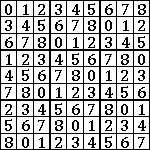
\includegraphics[width=0.6\linewidth]{sudoku_s_0.pdf}
\caption{Complete $S_0$ Sudoku for $n = 3$. The construction is defined in Proposition~\ref{prop:s_0}.}
\end{figure}

\begin{lemma}[\cite{takayuki2003complexity}]
\label{lem:sudoku_reduction}
Let $S$ be a Sudoku instance of order $n$ such that
\begin{displaymath}
S(i,j) = \left\{
\begin{array}{lr}
\perp & : (i,j) \in B\\
S_0 (i,j) & : \text{otherwise}
\end{array}
\right.
\end{displaymath}
where $B = \{ (i,j) | i < n \text{ and } (j \equiv 0) \mod n \}$. Let $S'$ be the Sudoku obtained by filling in the blanks of $S$. Then $S'$ is a correct Sudoku solution if and only if the following conditions hold:
\begin{itemize}
\item For any $(i,j) \in B$, $S'(i,j) \equiv 0 \mod n$
\item A square $L$ defined by $L(i, j/n) = S'(i,j)/n$ for all $(i, j) \in B$ is a complete Latin Square.
\end{itemize}
\end{lemma}

The proof of Lemma~\ref{lem:sudoku_reduction} is also in \cite{takayuki2003complexity}. Figure~\ref{fig:latinsquare_to_sudoku} shows how the Latin Square corresponds to certain sections of the Sudoku puzzle for $n=3$. The three columns of the Latin square are mapped to the parts of columns of the Sudoku. In the mapping,the values are scaled by $n$. 

\begin{figure}
\centering
\label{fig:latinsquare_to_sudoku}
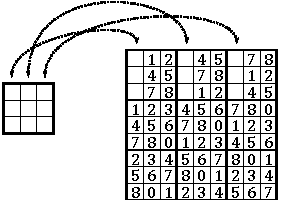
\includegraphics[width=0.7\linewidth]{latinsquare_to_sudoku.pdf}
\caption{Latin square taken from parts of $S_0$.}
\end{figure}

Lemma ~\ref{lem:sudoku_reduction} gives us the reduction from Latin Square to Sudoku. Given a Latin Square, we can create a Sudoku instance $S$ from the lemma. This is the reduction from \cite{takayuki2003complexity}.

\begin{lemma} 
$\mathsf{FCP}$ Sudoku is $\Sigma_2$-complete.
\end{lemma}

\begin{proof} 
We will show a general clue reduction via $\mathsf{FCP}$ Latin Squares. We use the injective map from instances of Latin Square to instances of Sudoku described in Lemma~\ref{lem:sudoku_reduction}. Let $C_B$ be the set of set of clues of Sudoku. We define $g$, by mapping a clue of Sudoku indicating that location $(i,j)$ contains $S(i,j)$ to the clue saying that the $(i, j/n)$ position of the Latin Square is $S(i, j)/n$. 
\begin{enumerate}
\item $g$ is surjective. Each Latin Square clue came from a clue of Sudoku.
\item $g$ is bijective on solutions. Each solution to Sudoku gives a solution to Latin Squares, and the solution is unique since all other numbers are parts of the instance. 
\item $g$ maps each clue to another clue. So subsets are always preserved. $c \subset c' \iff g(c) \subset g(c')$. 
\item $g$ maps each clue to one clue. So $|c| = |g(c)|$. 
\end{enumerate}
. Therefore, $\mathsf{FCP}$ Sudoku is $\Sigma_2$-complete. 
\end{proof}

\section{$\mathsf{FCP}$ Versions of Easy Problems}
\label{sec:easyproblems}

We would like to be able to understand what happens to problems in general when their $\mathsf{FCP}$ versions are asked.

\subsection{Connection to Counting Problems}

For any search problem, the related counting problem asks for the number of valid solutions. We suspect that problems in $\mathsf{P}$ with $\sharp \mathsf{P}$-hard counting problems also have hard $\mathsf{FCP}$ versions.

\subsection{$\mathsf{FCP}$ 2SAT} 


In this section, we consider the $\mathsf{FCP}$ version of the 2-satisfiability ($2SAT$) problem. The problem, which gives a 2-CNF Boolean formula and asks for a satisfying assignment, has a known polynomial time solution. However, the \emph{counting} version of the problem is a well-known $\sharp \mathsf{P}$-complete problem. In this section, we show $\mathsf{FCP}-2SAT$ is $\mathsf{NP}$-complete, lending credence to the idea that $\sharp \mathsf{P}$-hardness and $\mathsf{FCP}$-hardness are related. Formally, $\mathsf{FCP}-2SAT$ is formulated as follows.

\begin{quote}
\textbf{Instance}: A 2-CNF Boolean formula $\phi$ on variables $x_1, ..., x_n$. \\
\textbf{Question}: Does there exist a setting of $k$ variables so that the remaining formula is uniquely satisfiable?
\end{quote}

\begin{proposition}
$\mathsf{FCP} 2SAT$ is in \NP.
\end{proposition}

\begin{proof}
The clue of size $k$ is the certificate. Since $2SAT$ can be satified in polynomial time, we can check whether there is a unique solution in polynomial time.
\end{proof}

\begin{theorem} 
$\mathsf{FCP} 2SAT$ is \NP-hard.
\end{theorem}

We reduce from the NP-hard problem of determining whether a graph has an independent dominating set of size at most $k$ (MIDS). The problem gives a graph $G = (V,E)$ and asks for the smallest subset of vertices $S \subseteq V$ such that $S$ is an independent dominating set and $|S| \leq k$. In other words, such a set $S$ has the property that every vertex has a vertex in $S$ adjacent to it (dominated), and does not include any vertex pairs $u$ and $v$ where $(u,v)$ is an edge in the graph (independent). \\

\noindent\textbf{Problem:} Given a graph $G = (V, E)$. Does there exist $S \subset V$, with $|S| \leq k$ such that 
\begin{itemize}
\item $\forall v \in V$, either $v \in S$ or $(u, v) \in E$, $u \in S$ 
\item $u, v \in S$ implies that there is no edge between $u$ and $v$. 
\end{itemize}

The reduction works as follows. For each edge $(u,v)$, we add the constraint $(\neg u \vee \neg v)$ to the 2SAT formula. We claim that a clue set for the resulting 2SAT formula where all clues set variables to be true can be transformed into an independent dominating set of size $k$. For the backwards direction, we claim that an independent dominating set of size $k$ can be turned into a clue set of size $k$. 

%
%We claim that a clue set for the resulting 2SAT formula consists of a setting of $k$ variables to be true, and that the variables in the clue correspond to a minimum independent dominating set. For the other direction, we claim that a minimum independent dominating set gives us a minimum clue set for the 2SAT formula, by simply setting all the variables corresponding to vertices in the set to be true.

In order to restrict our attention to clues that set variables to be true, we need the following lemma.

\begin{lemma} Given a set of clues of size $k$ with $k_f > 0$ variables set to false, there exists another set of clues of size at most $k$ with strictly fewer than $k_f$ variables set to false.
\end{lemma}

\begin{proof} 
Consider a variable $x_i$ set to be false. Consider its set of neighbors $N(x_i)$, guaranteed to be non-empty via construction. First, consider the case where $N(x_i)$ contains nodes set to true. For each of the nodes $v \in N(x_i)$ that are set to true, a clue must either say that $v$ is true, or there must be a clue that implies that $v$ is true. No matter what, we can either remove $x_i$ or replace $x_i$ with a clue that one of its neighbors are true (CHECK THIS). It remains to consider the case where all the neighbors of $x_i$ are set to false. In this case, we can switch the clue that $x_i$ is set to false with a clue that $x_i$ is set to true, which will imply that all of its neighbors are false.
\end{proof}

Now, we show that a clue assignment gives an independent dominating set of the same size. Suppose we have a clue assignment of size at most $k$. We first apply the lemma above repeatedly until there are no false clues. So if we have a variable that is part of the clue, it is set to be true and implies all of its neighbors are false. Thus, we get independence because we cannot have two adjacent variables set to true. We have a dominating set as well, since if there exists a vertex where no neighbor is a clue, then we cannot possibly know that any neighbors are set to true (since clues can only imply that other vertices are false), and since true variables are the only ones that give implications, we cannot know what this vertex is. 

Now we show that an independent dominating set gives a clue assignment of the same size. Suppose we have a minimum independent dominating set. If we set each variable in the minimum independent dominating set to be true, then we know due to the fact that it is a dominating set that every variable will be implied. So we know that this is a valid clue set.

Ideally, we would like to generalize what we've shown above. One particular question is whether the $\mathsf{FCP}$ versions of problems with polynomial time algorithms have a better upper bound than $\Sigma_2$. In general the answer is no. Consider the following example:
\[ L = \{ \phi' = \phi \vee \left( \bigwedge_i x_i \right) | \phi \text{ is a Boolean formula }\} \]
Clearly, $L \in P$. Since on each input, we check whether the Boolean formula takes the following form, and if so, we accept. The clause with all variables being $1$ indicates that the formula has a satisfying assignment. In addition, the search problem for finding a satisfying assignment also has a polynomial time algorithm. We simply set all variables to $1$. However, what happens to the $\mathsf{FCP}$ version?

$\mathsf{FCP} L$ 
\begin{quote}
\textbf{Instance}: a Boolean formula $\phi \vee \left( \bigwedge_i x_i\right)$, along with a $k$.\\
\textbf{Question}: Is there a partial assignment of at most $k$ variables such that the remaining formula is a unique satisfying solution?
\end{quote}

\begin{proposition}
$\mathsf{FCP} L$ is co\NP-hard.
\end{proposition}

\begin{proof}
We can reduce from $\overline{SAT}$. 
\begin{align}
\phi \in \overline{SAT} &\leftrightarrow \forall x \phi(x) = 0 \\
				    & \leftrightarrow \langle (\phi \wedge \overline{z}) \vee \left(z \wedge \bigwedge_i x_i \right), 0 \rangle \in \mathsf{FCP} L
\end{align}
\end{proof}

Alternatively, we could look at another contrived language:
\[ L' = \{ \phi' = (\phi \wedge \overline{z}) \vee z | \phi \text{ is a Boolean formula and $z$ does not appear in $\phi$} \} \]
So $L' \in P$ and the search problem also has a polynomial time algorithm. However, it seems like $\mathsf{FCP} L'$ should be able to analyze what happens inside $\phi$. 

\begin{proposition}
$\mathsf{FCP} L'$ is $\Sigma_2$-complete. 
\end{proposition}

\begin{proof}
We reduce from $\mathsf{FCP} SAT$. If $\phi$ has a partial assignment of size at most $k$ with a unique solution, then $\phi' = (\phi \wedge \overline{z}) \vee z$ has a partial assignment of size at most $k+1$ with a unique solution. We simply add the assignment for variable $z$. 

If $\phi$ has no satisfying assignment, then $\phi'$ requires $n$ clues for a partial assignment with a unique solution. If $\phi$ has a partial assignment, but it requires more than $k$ clues, then if $\textbf{x}$ is a particular satisfying assignment to $\phi'$, if $z  \in \textbf{x}$, then $\textbf{x}$ needs at least $n$ solutions to be specified, if $\overline{z} \in \textbf{x}$, then we must specify $\overline{z}$ in the clue, and by assumption we must specify more than $k$ variables. Therefore, if $\phi$ needs more than $k$ clues, $\phi'$ will need more than $k+1$ clues. 
\end{proof}

\subsection{What can we say about easy languages?}

NEED TO FORMALIZE THIS A BIT MORE.

We can say something about a particular set of easy problems. 
\begin{proposition}
Suppose $A$ in a search problem with a polynomial time algorithm. Furthermore, suppose $x$ is an instance of $A$. If $c$ is some clue for $x$ and $x \cup c$ is another instance of $x$, then $\mathsf{FCP} A \in \NP$. 
\end{proposition}

\begin{proof}
The certificate is the clue, along with the solution. We only need to specify that the clue is the required size, the solution corresponds to the clue, and that there is a unique solution. We do this by showing by asking whether $x \cup c \cup \{ c' \}$ has a solution for each possible additional clue $c'$ (for which there are polynomially many). If we can find more than one solution, we reject. If there is only one solution, we accept. Since $x \cup c \cup \{ c' \}$ is an instance to $A$, and $A$ has a polynomial time algorithm, we can verify that $c$ is a clue with a unique solution in polynomial time.
\end{proof}

We know that many polynomial time problems which we care about satisfy the above self-reducibility property. These include 2SAT, Horn-satisfiability, and matching. The languages $L$ and $L'$ do not satisfy the above properties.

\section{Conclusion}
\label{sec:conclusion}


\bibliography{references}
\bibliographystyle{splncs}
\end{document}
